%%%%%%%%%%%%%%%%%%%%%%%%%%%%%%%%%%%%%%%%%%%%%%%%%%%%%%%%%%%%%%%%%%%%
%%%%%                         HEADER                           %%%%%
%%%%%%%%%%%%%%%%%%%%%%%%%%%%%%%%%%%%%%%%%%%%%%%%%%%%%%%%%%%%%%%%%%%%
%%%%%                Author : Coraline Marie                   %%%%%
%%%%%%%%%%%%%%%%%%%%%%%%%%%%%%%%%%%%%%%%%%%%%%%%%%%%%%%%%%%%%%%%%%%%


\documentclass[a4paper]{article}


%%%%% Packages %%%%%

	%%%%% Langage %%%%% 
\usepackage[frenchb]{babel}
\usepackage[utf8]{inputenc}
\usepackage[T1]{fontenc}
	%%%%% Graphique %%%%%
\usepackage{graphicx}
\usepackage{wrapfig}
	%%%%% Mise en page %%%%%
\usepackage{hyperref}
\usepackage{fancyhdr}
\usepackage{colortbl}


%%%%% Macros %%%%
%%%%%%%%%%%%%%%%%%%%%%%%%%%%%%%%%%%%%%%%%%%%%%%%%%%%%%%%%%%%%%%%%%%%
%%%%%                         MACROS                           %%%%%
%%%%%%%%%%%%%%%%%%%%%%%%%%%%%%%%%%%%%%%%%%%%%%%%%%%%%%%%%%%%%%%%%%%%
%%%%%                Author : Coraline Marie                   %%%%%
%%%%%%%%%%%%%%%%%%%%%%%%%%%%%%%%%%%%%%%%%%%%%%%%%%%%%%%%%%%%%%%%%%%%


%%%%% Ligne de séparation %%%%%
\newcommand{\HRule}{\rule{\linewidth}{0.5mm}}


%%%%% Recoloration des liens %%%%%
\hypersetup{colorlinks = true,
            breaklinks = true,
            linkcolor = {blue},
            urlcolor = {blue},}


%%%%% Création de nouvelles couleurs %%%%%
\definecolor{lightgray}{rgb}{0.75,0.75,0.75}


%%%%% Saut de ligne %%%%%
\newcommand{\NewLine}{\vspace{0.5cm}}


%%%%% Inclusion d'en-tête %%%%%
\pagestyle{fancy}
\setlength{\headheight}{23pt}	% Correction du warning \headheight is too small
\lhead{Coraline \textsc{Marie}}
\rhead{Link Inter Message Detector}


%%%%%%%%%%%%%%%%%%%%%%%%%%%%%%%%%%%%%%%%%%%%%%%%%%%%%%%%%%%%%%%%%%%%
%%%%% DOCUMENT %%%%%
%%%%%%%%%%%%%%%%%%%%%%%%%%%%%%%%%%%%%%%%%%%%%%%%%%%%%%%%%%%%%%%%%%%%

\begin{document}

	%%%%% Page de garde %%%%%
	%%%%%%%%%%%%%%%%%%%%%%%%%%%%%%%%%%%%%%%%%%%%%%%%%%%%%%%%%%%%%%%%%%%%
%%%%%                    PAGE DE GARDE                         %%%%%
%%%%%%%%%%%%%%%%%%%%%%%%%%%%%%%%%%%%%%%%%%%%%%%%%%%%%%%%%%%%%%%%%%%%
%%%%%                Author : Coraline Marie                   %%%%%
%%%%%%%%%%%%%%%%%%%%%%%%%%%%%%%%%%%%%%%%%%%%%%%%%%%%%%%%%%%%%%%%%%%%

\begin{titlepage}
	\begin{center}

		%%% Logo et sous-titre
		
\includegraphics[width=0.35\textwidth]{Figures/ATAL.png}~

		\LARGE{Master 2 \textsc{ATAL}}\\[1.5cm]

		\Large{Développement de logiciels et de projets}\\[0.5cm]

		%%% Titre
		\HRule \\[0.4cm]
		{ \huge \bfseries Link Inter Message Detector \\[0.4cm] }
		\HRule \\[1.5cm]

		%%% Auteurs et professeur
		\normalsize		
		\emph{\'Etudiante :}\\
		Coraline \textsc{Marie}

		\vspace{0.5cm}

		\emph{Encadrant :} \\
		Nicolas \textsc{Hernandez}

		\vspace{1cm}

		%%% Date de rendu
		{\large 5 janvier 2015}

		\vfill

		
		
\includegraphics[width=0.35\textwidth]{Figures/logoUN.png}~\\[2cm]

		

	\end{center}
\end{titlepage}




	%%%%% Sommaire %%%%%
	\tableofcontents
	\newpage

	%%%%% Introduction %%%%%
	\section*{Introduction}
	\addcontentsline{toc}{section}{\protect\numberline{}Introduction}
	
	UIMA (Unstructured Information Management Architecture) est un framework  capable d'analyser de grands volumes de données non structurées, et d'identifier des informations pertinentes pour un utilisateur lambda. Cette technologie a été créée par IBM, et est actuellement enseignée au Master 2 ATAL de l'Université de Nantes.\\

	\textbf{Link Inter Message Detector} est un travail réalisé dans le cadre du cours \textit{"Développement de logiciels et de projets"}. Ce projet a pour objectif de détecter automatiquement les liens entre plusieurs messages désorganisés, en utilisant le framework UIMA.\\

	Ce rapport présente donc le résultat de ce travail, avec l'explication de mes choix d'implémentations et mes résultats. Nous étudierons d'abord la conception du programme puis son implémentation, avant de finir par son utilisation.


	%%%%% Parties 1 %%%%%
	
	\section{Conception}
	
	L'objectif de ce projet est de trouver des liens entre plusieurs messages désorganisés appartenant à un même thread. Pour ce faire, le programme a été divisé en deux grandes étapes. Tout d'abord, on construit un réseau de collocation à partir d'une archive html d'Ubuntu. Ensuite, on construit pour chaque message d'un autre corpus (Zim), une ou plusieurs chaînes lexicales. Pour finir, on compare ces messages entre-eux grâce à leurs chaînes lexicales afin de trouver des correspondances et donc, des liens entre les messages.\\
	
	Afin d'accélérer la conception de ce projet, plusieurs ressources ont été fournies en même temps que le sujet :
\begin{itemize}
	\item une archive contenant de la documentation Ubuntu : Zim;
	\item un fichier contenant des mails de la liste de diffusion d'Ubuntu : Mbox; 
	\item une liste de mots outils : stopwords;
	\item un fichier contenant les threads de discussion du Mbox : Digest.
\end{itemize}

	\subsection{Initialisation du projet}
	
	Avant même de commencer à coder le programme, il faut d'abord imaginer son architecture. Pour ma part, j'ai d'abord fait plusieurs schémas avant de réussir à définir la structure du programme. La figure 1 décrit la première version de l'architecture de mon programme. Celle-ci était divisée en trois Workflows : la création du réseau de collocation, la création des chaînes lexicales et la comparaison. Le dernier workflow est encore flou sur ce schéma car je ne savais pas encore comment le faire avant de commencer à coder. \\
	
	\begin{figure}[!]
  	\centering
  	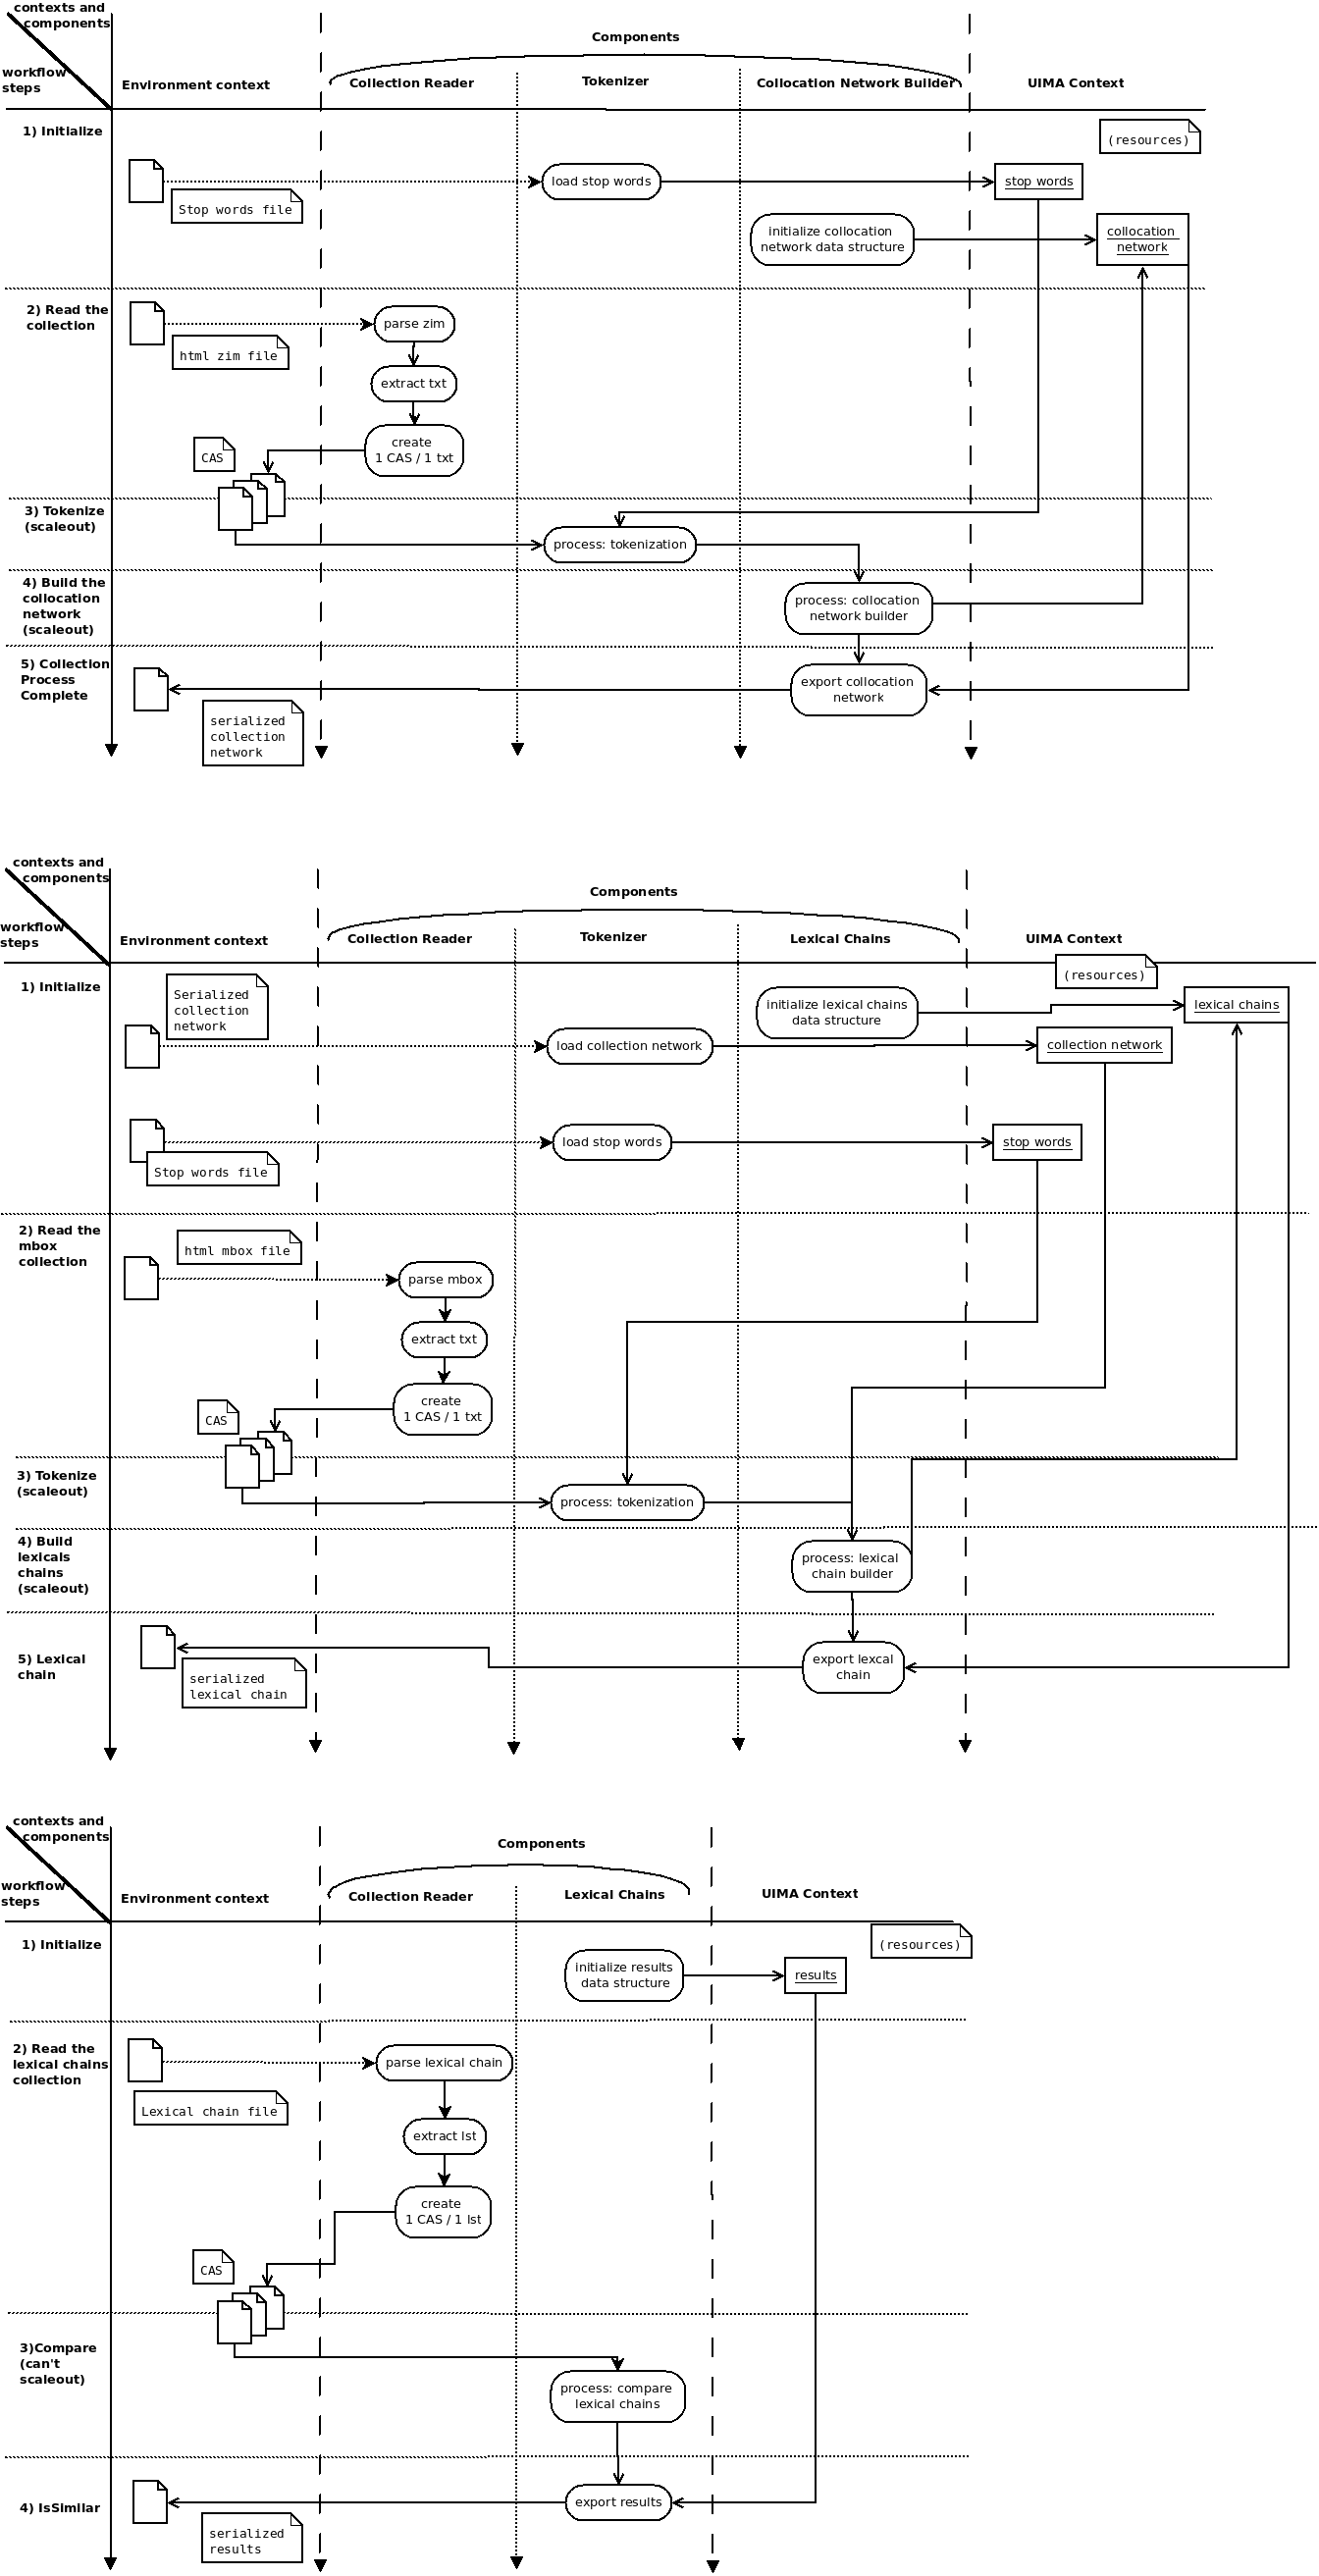
\includegraphics[width=1\textwidth]{Figures/mondiagramme1.png}
  	\caption{Premier diagramme}
	\end{figure}
		
Les figures 2 et 3 sont les dernières versions de l'architecture. Ce sont celles que j'ai suivi pour coder le programme définitif. Il y a maintenant deux workflows, le premier pour la création du réseau de collocation, et le deuxième regroupe la construction des chaînes lexicales et la comparaison des messages.
	
	\begin{figure}[!]
  	\centering
  	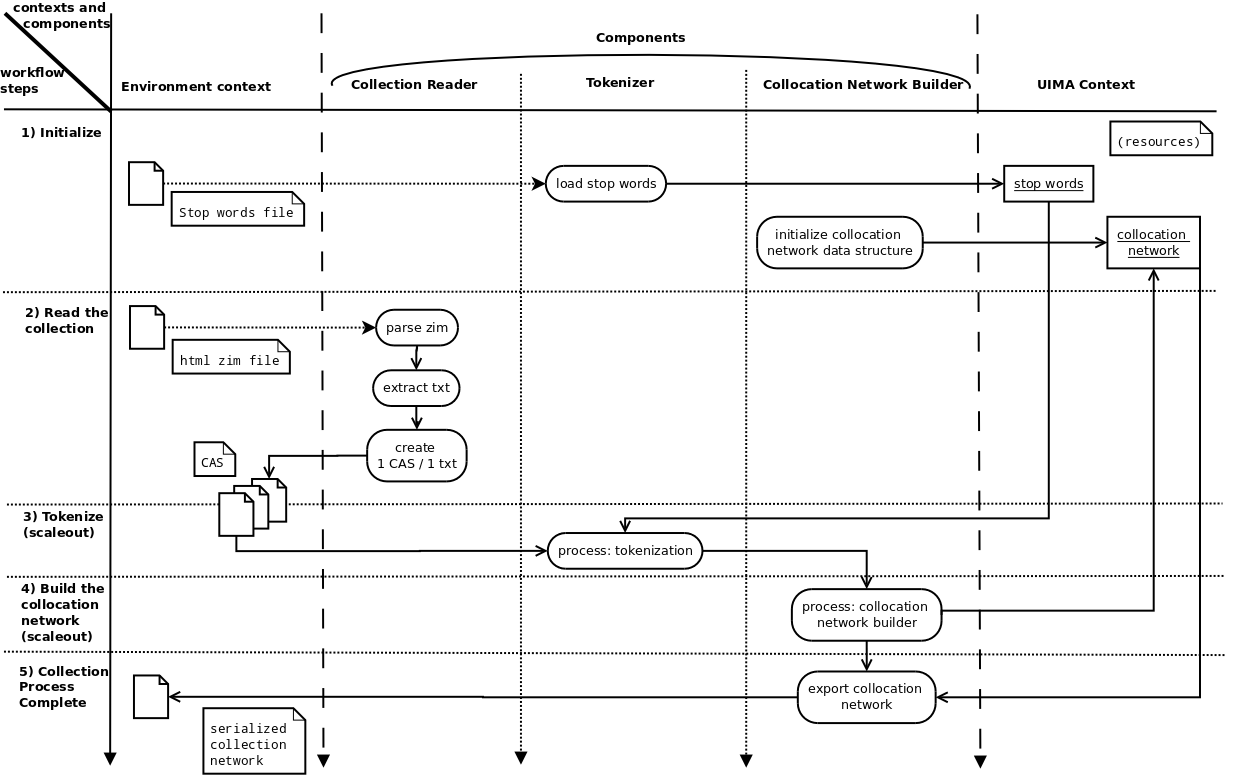
\includegraphics[width=1\textwidth]{Figures/cn.png}
  	\caption{Dernier diagramme : collocationNetwork}
  	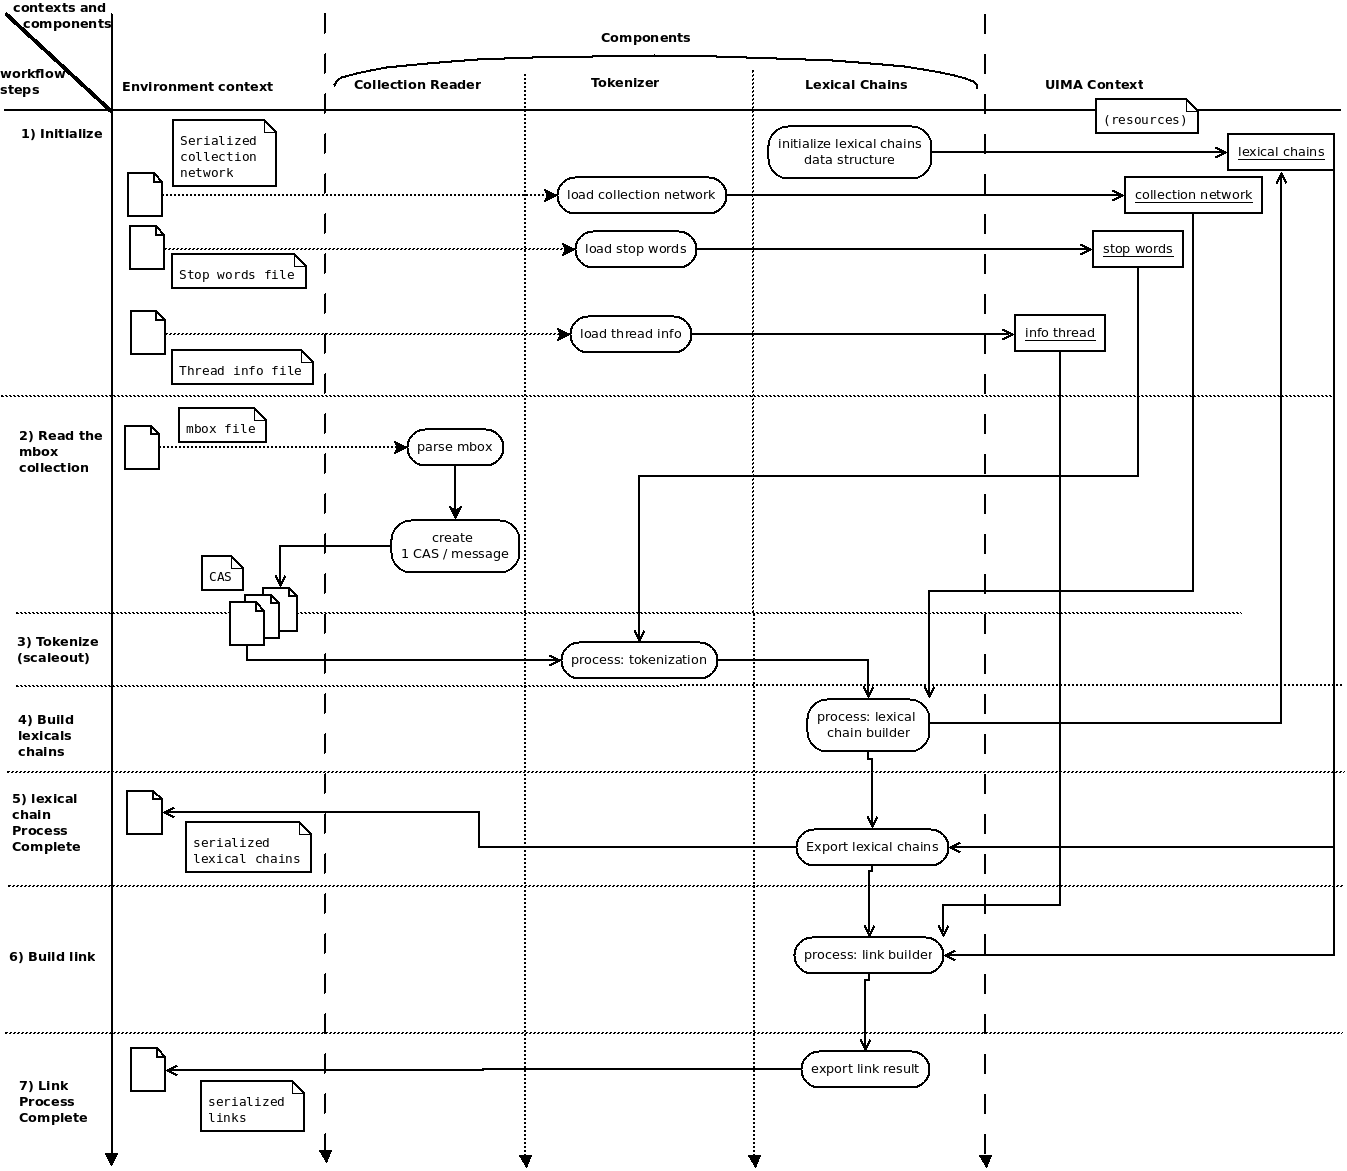
\includegraphics[width=1\textwidth]{Figures/mondiagramme.png}
  	\caption{Dernier diagramme : linkDetection}
	\end{figure}
	
	
	\subsection{Construction du réseau de collocation}
	
	Le premier workflow créé fut celui du réseau de collocation. En effet, la première étape du programme consiste à utiliser un corpus Zim comme corpus d'apprentissage, afin de créer un réseau de collocation. Ce corpus est différent de celui avec lequel nous manipulerons les messages dans la suite du programme. Il s'agit d'une documentation pour Ubuntu, datée de 2009. Pour coder la création du réseau de collocation, j'ai suivi scrupuleusement le diagramme fourni avec les sources (figure 2). Sur ce schéma, on peut voir que ce workflow utilise deux "Analysis Engine". Le premier tokénize le texte à l'aide des ressources fournis dans le wordSegmenter. Le deuxième créé toutes les paires de collocations, puis il les sauvegarde dans une nouvelle ressource "collocationNetwork.tsv".

	\subsection{Détection de liens entre les messages}

	Le second workflow créé, utilise des chaînes lexicales pour détecter les liens entre les messages. Pour ce faire, un deuxième corpus a été fourni : le Mbox. Ce corpus contient un ensemble de messages récupéré sur le forum d'Ubuntu. Il traite donc du même sujet que le premier corpus qui nous a permis d’établir le réseau de collocation. La figure 3 détaille le fonctionnement de cette partie du programme. Tout d'abord, les messages sont extraits un par un, ce qui permet d'obtenir un CAS par message. Ensuite, chaque message est tokenisé exactement comme dans le premier workflow. Une fois la segmentation terminée, on construit des chaînes lexicales pour chaque message à partir du réseau de collocation. Puis on utilise ces chaînes lexicales pour comparer les messages entres eux et détecter des liens.
	
	\section{Implémentation}

Le programme a été codé sur Eclipse à partir de l'archive et des exemples de code fournis avec le sujet du projet. Afin d'utiliser au mieux les ressources fournies, j'ai conservé le packaging proposé. Je vais donc présenter les éléments package par package pour plus de simplicité dans la lecture du code. 

	\subsection{zim2collocationNetwork}
	Le package \texttt{zim2collocationNetwork} contient tous les objets java que j'ai créé ou modifié pour permettre la génération du réseau de collocation. L'Analysis Engines \texttt{CollocationNetworkBuilderAE} a été partiellement fourni, il ne manquait que la partie process à coder.

	\subsection{mbox2lexicalChain}
	Le package \texttt{mbox2lexicalChain} a été fourni pour aider notamment à la tokénisation des messages. On y trouve donc l'Analysis Engines \texttt{MBoxMessageParserAE} qui permet de découper le corpus en messages. J'ai d'ailleurs rajouté le type Message afin de garder certaines informations comme l’Id du message, nécessaire pour la suite du programme. Cet AE est lancé dans le second workflow, avant l'AE de segmentation, ce qui permet de tokeniser uniquement le corps du message.

	\subsection{linkDetection}
	Ce package ne contient que des objets Java que j'ai créé pour le second workflow. Ils permettent de créer les chaînes lexicales et de faire la comparaison des messages. L'Analysis Engines \texttt{LexicalChainsNetworkBuilderAE} s’inspire des travaux de Marathe \& Hirst pour créer des chaînes lexicales et pour les évaluer. Cependant si plusieurs chaînes lexicales obtiennent de bons scores, on ne garde que la meilleure chaîne. Les scores de similarité qui permettent de déterminer si un mot appartient à une chaîne lexicale étant calculés par moyenne, il est peu probable d’obtenir plusieurs chaînes avec le score optimal. Dans la méthode de Marathe \& Hirst, pour un mot donné, toutes les chaînes déjà calculées sont candidates. Mais cela demandait trop de ressources pour mon ordinateur, je me suis donc limité en ne gardant pour candidats que les 20 dernières chaînes. Cela réduit mes résultats, mais mon netbook avec Eclipse ne disposait pas d'assez de mémoire pour arriver au bout du processus. L'Analysis Engines \texttt{LinkerAE} s'éxecute juste après. Il utilise également les informations du thread décrites ci-après. La détection des liens se fait message par message, sans avoir créée à l'avance toutes les chaînes lexicales de tous les messages. Cela signifie que pour un message donné, on regarde les autres messages de son thread et on choisit celui qui est le plus proche. La similarité entre deux messages est ensuite calculée d’après la moyenne des similarités entre les chaînes lexicales les composant.

	\subsection{wordSegmenter}
	Le package \texttt{wordSegmenter} contient tous les objets java qui ont été fournis pour permettre la segmentation des corpus. L'Analysis Engines \texttt{WordSegmenterAE} a été fourni et n'a pas subi de modifications.

	\subsection{Les ressources}
	La première ressource importante est le Stop Words. Celle-ci était fournie et permet d'éliminer les mots outils lors de la segmentation des corpus. 
La seconde ressource est le réseau de collocation. Celle-ci est initialisée et remplie lors du l'execution du premier workflow. Elle est constituée de paires de mots pour lesquelles on a associé un score de collocation. Cette ressource est notamment utilisée lors de l'éxecution du deuxième workflow pour la création des chaînes lexicales. 
Les chaînes lexicales forment la troisième ressource. Elle est donc créée lors de l'éxecution du deuxième workflow et contient les identifiants de chaque message auquel on a associé l'ensemble des chaînes lexicales représentant ce même message. 
Les informations sur les thread sont une ressource qui s’appuie sur les informations disponibles dans un fichier thread digest. Elle détaille la structure des threads et stocke chaque thread avec les messages qu’il contient, ainsi que chaque message avec le thread auquel il est associé. Cette redondance permet par la suite d’accéder plus rapidement aux informations nécessaires. Cette ressource a été mise en place par les M2 Atal de l'année dernière, je l'ai donc reprise et modifiée afin de pouvoir l'intégrer dans mon code.
	
	
	\section{Utilisation du programme}

	L'intégralité de mon code se trouve sur mon GitHub : \url{https://github.com/Slayerxoxo/myUimaDevLogProject}\\
	
Cependant, les corpus n'y sont pas car ils sont trop lourds. Ces derniers doivent être rajoutés dans un dossier data, et certains liens devront être modifiés pour la bonne exécution du programme. Le code a été fait sous Eclipse mais il peut également être utilisé via Maven. 

L'exécution du programme complet se fait par le lancement des deux workflow : d'abord le CollocationNetworkBuilderWF.java, puis le MboxWF.java.


	%%%%% Conclusion %%%%%
	\section*{Conclusion}
	\addcontentsline{toc}{section}{\protect\numberline{}Conclusion}

	Au terme de ce travail, plusieurs remarques peuvent être faites. Tout d'abord, notons que ce projet nous a permis de découvrir une nouvelle technologie : UIMA. Bien que l'utilisation de ce framework ne soit pas facile à apprendre, à terme il s'est révélé être un outil puissant et très utile pour le traitement automatique des langues. 

	Cependant, UIMA reste un framework Java, ainsi beaucoup de tâches qui seraient rapides à coder dans un langage de script tel que le Python ou le Perl, sont lentes et laborieuses à écrire en Java. De plus, il existe assez peu de documentation et d'explications sur Internet.

	\subsection*{Résultats}
	Ce travail avait pour principal objectif d'apprendre à se servir de UIMA, ce qui m'a pris pas mal de temps, j'ai donc délaissé le côté évaluation que j'aurais bien aimé approfondir. Malheureusement je n'ai jamais réussi à aller jusqu'au bout du programme. Le code que j'ai écrit n'est pas optimisé et je me suis rendu compte assez tard que le corpus était très pollué (pièce jointes, images,\dots). Il aurait fallu que je code un script pour nettoyé le corpus pour pouvoir travaillé correctement sur l'intégralité du corpus, mais j'ai manqué de temps. Les résultats que j'ai obtenu sont tirés d'une version allégée du corpus qui a été créée par les anciens M2 Atal. Ils ne sont donc pas représentatif du corpus complet et sont assez mauvais. L'évaluation des résultats c'est faite par l'intermédiaire d'un programme Perl fourni : P = 0.4550 et R = 0.0285. 

	%\newpage
	
	%%%%% Bibliographie %%%%% (Attention, citer une source de bibliographie sinon bug)
	%\bibliographystyle{plain}
	%\bibliography{biblio}

\end{document}
